% 2026年北京高考数学第14题：三棱锥A-BCD
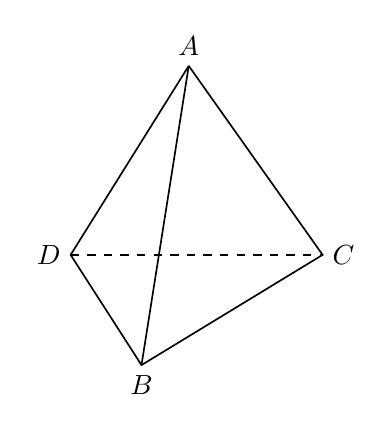
\begin{tikzpicture}[>=stealth,line width=0.6pt,font=\normalsize]
  \coordinate (A) at (1.5,3.2);
  \coordinate (D) at (0,0.8);
  \coordinate (B) at (0.9,-0.6);
  \coordinate (C) at (3.2,0.8);

  % 实线可见边
  \draw (A) -- (D) -- (B) -- (C) -- (A);
  \draw (A) -- (B);

  % 虚线不可见底边
  \draw[dashed] (D) -- (C);

  % 顶点标注
  \node[above] at (A) {$A$};
  \node[left] at (D) {$D$};
  \node[below] at (B) {$B$};
  \node[right] at (C) {$C$};
\end{tikzpicture}
